\section{Scelte progettuali}
Di seguito verranno illustrate le principali scelte progettuali effettuate durante la realizzazione del progetto.

\subsection{Architettura del server}
\sloppy
L'architettura del server è stata scelta tra due soluzioni, che sono state trattate più in dettaglio durante il Laboratorio di Reti di Calcolatori:

\begin{enumerate}
	\item multithread sincrona con I/O bloccante (\texttt{Sockets} di \texttt{Java IO});
	\item monothread sincrona con I/O non bloccante (\texttt{Selectors} di \texttt{Java NIO}).
\end{enumerate}

Le due soluzioni hanno pregi e difetti complementari, ma il trade-off principale è tra \textbf{velocità} e \textbf{scalabilità}. Ai fini di questo progetto didattico è stata ritenuta più importante la reattività, garantita (sotto carichi non eccessivi) dalla prima soluzione.
\medskip \\
Possiamo dividere il server in due livelli: \textbf{interfaccia} e \textbf{core}.

\begin{enumerate}
	\item A livello di interfaccia si trovano:
		\begin{enumerate}
			\item Il socket TCP del server
			\item L'API del servizio di registrazione utente
			\item Il servizio RMI di notifiche push.
		\end{enumerate}
	\item A livello core si trovano:
		\begin{enumerate}
			\item Il thread pool di client handlers
			\item I manager di utenti, documenti e indirizzi IP multicast.
		\end{enumerate}
\end{enumerate}

Per ogni client che si connette, il server riserva un thread, che si occuperà di gestire la connessione TCP per l'intero tempo di vita del client.

\subsection{Comunicazione client-server}
Per la comunicazione client-server è stata adottata una tecnica a scambio di messaggi sincrona. I messaggi sono in formato JSON, e vengono inviati attraverso una connessione TCP. La scelta del formato JSON al posto degli oggetti Java serializzati può permettere in un futuro momento di scrivere client per \texttt{TURING} in qualsiasi linguaggio di programmazione\footnote{A patto di modificare leggermente la parte di registrazione di un nuovo utente, che è stata richiesta esplicitamente in Java RMI.}.

\newpage

\begin{center}
	\begin{figure}[h!]
		\makebox[\textwidth]{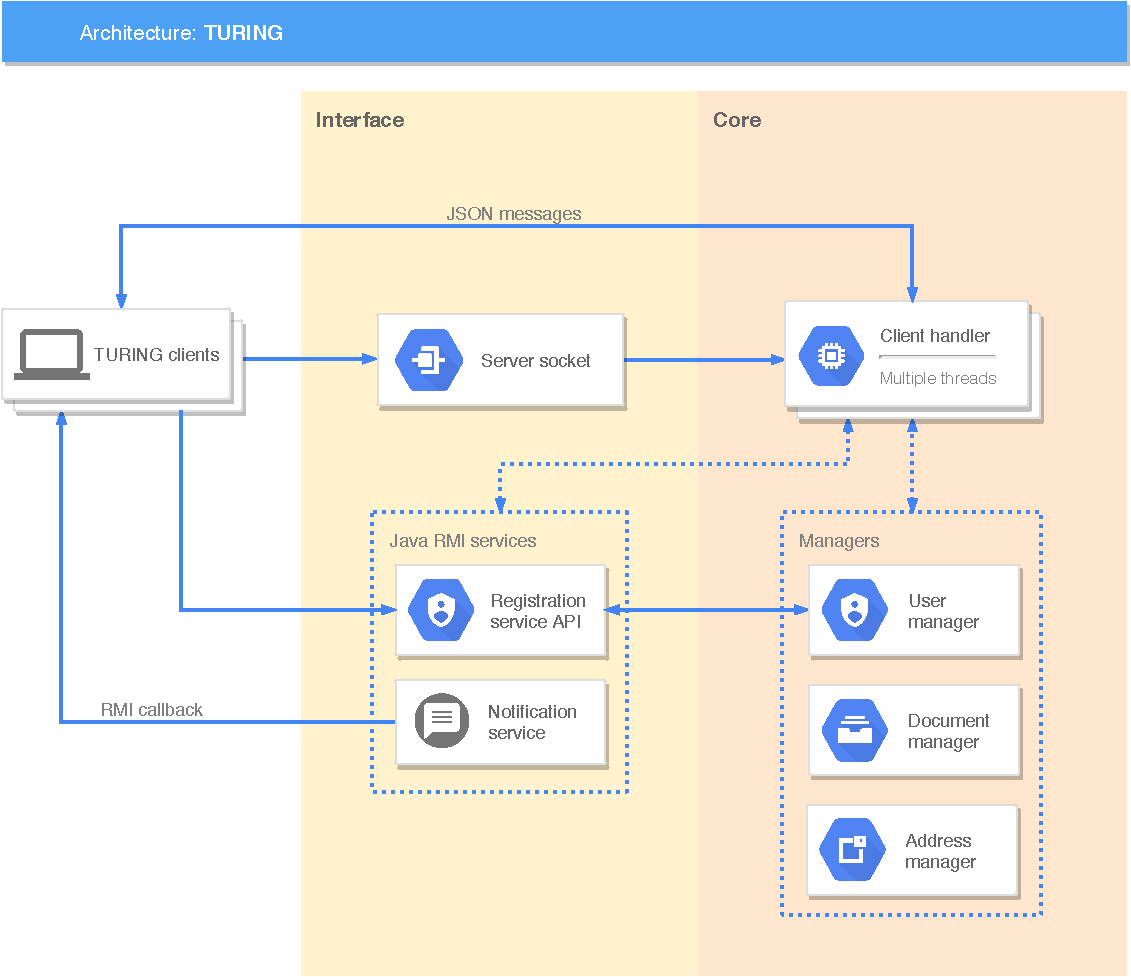
\includegraphics[width=0.75\paperwidth]{img/turing_architecture.pdf}}
		\caption{Architettura di \texttt{TURING} e interazioni tra le varie componenti.}
	\end{figure}
\end{center}

\subsection{Architettura del client}
L'architettura del client è più semplice: effettua richieste in formato JSON e resta in attesa di una risposta. Il thread grafico è aggiornato all'occorrenza dal metodo \textit{invokeLater}. L'interfaccia grafica si adatta automaticamente alle dimensioni dello schermo, ed è stato cercato di renderla il più coerente, gradevole e intuitiva possibile.

\medskip

Dalla schemata di registrazione e login si può accedere all'area personale di \texttt{TURING}, dove ogni utente può creare nuovi documenti, invitare altri utenti alla modifica, e in una tabella dinamica vede i documenti che può modificare, con la lista delle sezioni e informazioni aggiuntive, come il nome del creatore del documento (indispensabile nel caso di documenti omonimi) e un'icona che indica se il documento è stato condiviso o no. La tabella si aggiorna in tempo reale quando si viene invitati alla modifica di un nuovo documento (con apposito messaggio di notifica), ma è anche possibile forzare un aggiornamento manuale tramite il tasto ``refresh".

\medskip

Dopo che una sezione di un documento è stata selezionata per la modifica, viene visualizzata la schermata di lavoro, nella quale è possibile modificare il testo precedentemente salvato, chattare con gli utenti che stanno modificando lo stesso documento, salvare le modifiche o ignorarle. I documenti sono codificati nello standard \texttt{UTF-8}.

\medskip

Il formato dei messaggi è indicato nel file \texttt{message\_format.txt}, assieme ad un esempio di messaggio che richiede al server la creazione di un documento.
